
The event yields, as shown in Table~\ref{tab:eventYieldCTagEx}, have two types of uncertainties: 
statistical and systematics. For N number of events, the absolute statistical uncertainty is 
$\sqrt{\text{N}}$. The systematic uncertainties arise due to improper calibration of the detector, 
the uncertainty in the efficiency of the reconstruction algorithm, uncertainty difference in 
theoretical prediction etc. The systematics uncertainties considered in this analysis are 
divided into two categories: experimental and theoretical uncertainties.

\section{Experimental uncertainties}
\begin{itemize}[leftmargin=*]
\item {\bf{Luminosity}}: The uncertainty in the integrated luminosity is 2.5\% for 2016 data taking~\cite{CMS-PAS-LUM-17-001}. 
\item {\bf {Pileup reweighting}}: The pileup weights as discussed in Section~\ref{s:pileup_reweighting}
    are calculated using minimum bias cross-section 69.2\unit{mb}. The uncertainty in the minimum 
    bias cross-section affects the pileup distribution. The 
    minimum bias cross-section is varied up and down by 4.7\% and corresponding pileup
    weights are applied to simulated events. The effect of pileup uncertainty on the $\mjj$
    shape is shown in Figures~\ref{subfig:sys_Pileup_wh_mu},~\ref{subfig:sys_Pileup_wh_ele} and
    Figures~\ref{subfig:sys_Pileup_ttbar_mu},~\ref{subfig:sys_Pileup_ttbar_ele} for charged Higgs
    and \ttjets sample, respectively for both channels.

\item {\bf {Lepton trigger, tracking, identification and isolation}}: 
    The lepton scale factors as discussed in Section~\ref{s:lepton_sf} are applied to the simulated
    samples. A conservative 3\% uncertainty is considered on combined lepton scale factors
    for both channels. 

\item {\bf {Jet energy, \MET correction}}: The $\pt$ of jet in the simulation are corrected using JES 
    and JER as discussed in Section~\ref{s:JEC}. The jet correction is propagated to correct 
    \MET. The $\mjj$ shape are also affected by the uncertainties in the JES, JER as shown in 
    Figures~\ref{subfig:sys_JES_wh_mu},~\ref{subfig:sys_JES_wh_ele},~\ref{subfig:sys_JER_wh_mu},
    and \ref{subfig:sys_JER_wh_ele} for charged Higgs signal ($\mHp = 120$ \GeV) and in 
     Figures~\ref{subfig:sys_JES_ttbar_mu},~\ref{subfig:sys_JES_ttbar_ele} 
    ~\ref{subfig:sys_JER_ttbar_mu}, and \ref{subfig:sys_JER_ttbar_ele} for \ttjets 
    background for both channels. 

\item {\bf {\PQb and \PQc tagging uncertainty}}: The \PQb and \PQc jets are present within the same 
    event. The \PQb and \PQc tag scale factors (as described in Section~\ref{s:bTagSF} and 
	Section~\ref{s:cTagSF}) are correlated to each other as shown in Figure~\ref{fig:bcCorr}. 
    	The correlated scale factors are varied up/down simultaneously. Therefore, we have three
	systematic uncertainties from \PQb and \PQc tagging. Based on their grouping in 
	Figure~\ref{fig:bcCorr}, we have the following three nuisance parameters:
    \begin{figure}
    \begin{center}
    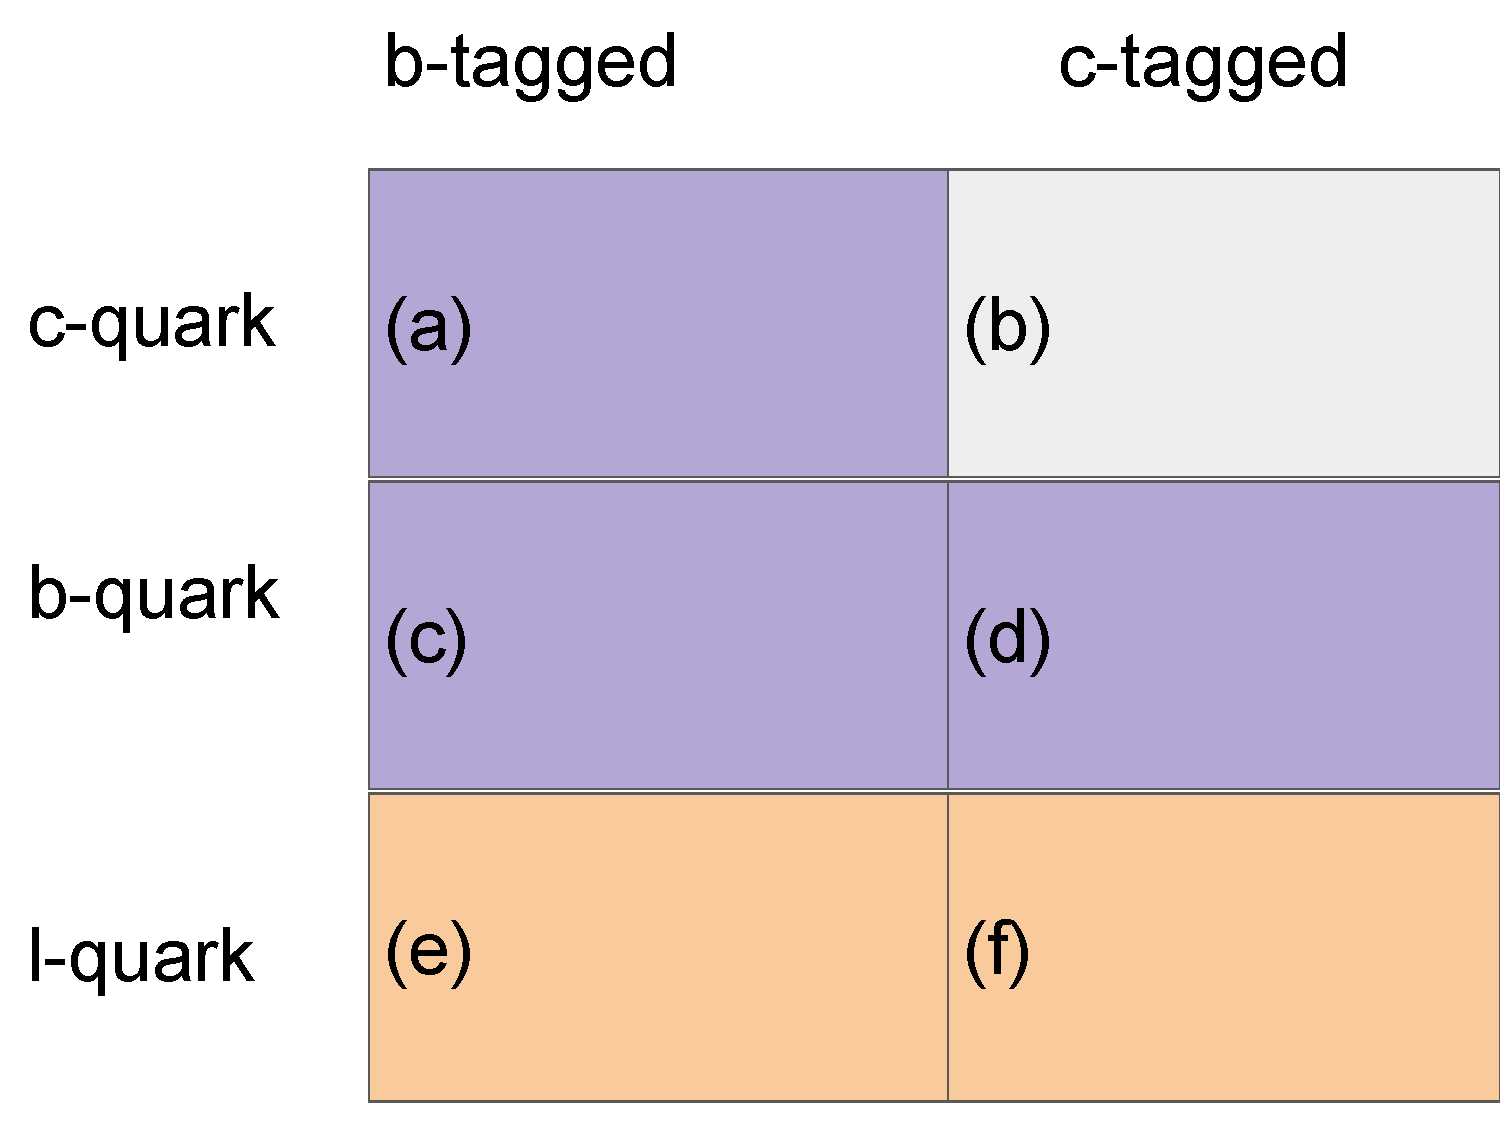
\includegraphics[width=0.50\textwidth]{Image/bcCorrelation.pdf}
    \caption{Correlation of \PQb and \PQc tag scale factors. In the region (a), \PQc quark is tagged 
	as \PQb jet; in region (b), \PQc quark is tagged as \PQc jet; in region (c), \PQb quark is 
	tagged as \PQb jet; in region (d), \PQb quark is tagged as \PQc jet; in region (e), light 
	quark is tagged as \PQb jet; and in region (f), light quark is tagged as \PQc jet.}
    \label{fig:bcCorr}
    \end{center}
    \end{figure}
    \begin{itemize}[leftmargin=*]
    \item \verb|CMS_eff_bcInc3| (correlating (a), (c), (d))
    \item \verb|CMS_eff_bcInc2| (correlating (e), (f))
    \item \verb|CMS_eff_bcInc1| (from (b))
    \end{itemize}
    After $\geq$ 1 \PQc jet selection, the effect of \PQb/\PQc tagging systematics on the shape 
	of $\mjj$ distribution are shown in    
    Figures~\ref{subfig:sys_bcTag1_wh_mu},~\ref{subfig:sys_bcTag2_wh_mu},~\ref{subfig:sys_bcTag3_wh_mu},
    and ~\ref{subfig:sys_bcTag1_wh_ele},~\ref{subfig:sys_bcTag2_wh_ele},~\ref{subfig:sys_bcTag3_wh_ele}
    for charged Higgs signal ($\mHp = 120$ \GeV) and in
    Figures~\ref{subfig:sys_bcTag1_ttbar_mu},~\ref{subfig:sys_bcTag2_ttbar_mu},~\ref{subfig:sys_bcTag3_ttbar_mu},
    and
    ~\ref{subfig:sys_bcTag1_ttbar_ele},~\ref{subfig:sys_bcTag2_ttbar_ele}~,\ref{subfig:sys_bcTag3_ttbar_ele}
    for \ttjets background for both channels.

    \item {\bf{Uncertainties for exclusive charm categories}}: The \PQc tag scale factors are
        officially not available for exclusive event categories. Therefore, conservatively, the
        inclusive scale factors are used for exclusive event categories. However, one extra systematic
        uncertainty is considered for exclusive categories. The mean of inclusive \PQc tag weights
        (Equation (\ref{eq:btagWt})) is calculated based on whether a jet is satisfying one of the 
        charm working points and not satisfying the other (\eg a jet satisfies loose and medium but 
        not tight working, as shown in Tables~\ref{tab:extraNPL},~\ref{tab:extraNPM}). The following
	two nuisance parameters are considered for exclusive categories. 
        \begin{itemize}[leftmargin=*]
        \item \verb|CMS_eff_ExL|: The ratio (max/min) of mean of inclusive c-tag weights from four
            combinations (yLyMyT, yLyMnT, yLnMyT, yLnMnT) is considered. 
        \item \verb|CMS_eff_ExM|: For exclusive medium charm category, the ratio (max/min) of
            event weights from two combinations (yMyT, yMnT) are considered. 
        \end{itemize}
    	The inclusive and exclusive event categories are same for tight charm working points, hence no
    	extra systematic uncertainty is considered. The loose and medium \PQc tag event weight 
	corresponding to Tables~\ref{tab:extraNPL}, \ref{tab:extraNPM} are shown in 
	Figure~\ref{fig:extraNP} for both channels, from \ttjets sample. Similar event weights are 
	found for simulated signal samples.
    \begin{table}
    \caption{Inclusive loose \PQc tag types. The acronym yLyMnT refers to the case where a jet
    satisfies loose and medium, but not tight working point.}
    \label{tab:extraNPL}
    \begin{center}
    \begin{tabular}{cccc}
    \hline
    \hline
    {\bf{Loose }} & {\bf{Medium }} & {\bf{Tight }} & {\bf{Acronym}} \\
    \hline
    \hline
    Y     & Y & Y & yLyMyT \\
    Y     & Y & N & yLyMnT \\
    Y     & N & Y & yLnMyT \\
    Y     & N & N & yLnMnT  \\
    \hline
    \end{tabular}
    \end{center}
    \end{table}

    \begin{table}
    \caption{Inclusive medium \PQc tag types.}
    \label{tab:extraNPM}
    \begin{center}
    \begin{tabular}{ccc}
    \hline
    \hline
    {\bf{Medium }} & {\bf{Tight }} & {\bf{Acronym}} \\
    \hline
    \hline
     Y & Y & yMyT \\
     Y & N & yMnT \\
    \hline
    \end{tabular}
    \end{center}
    \end{table}

    \begin{figure}
    \centering  
    \subfigure[\label{subfig:extraNPmu}]
    {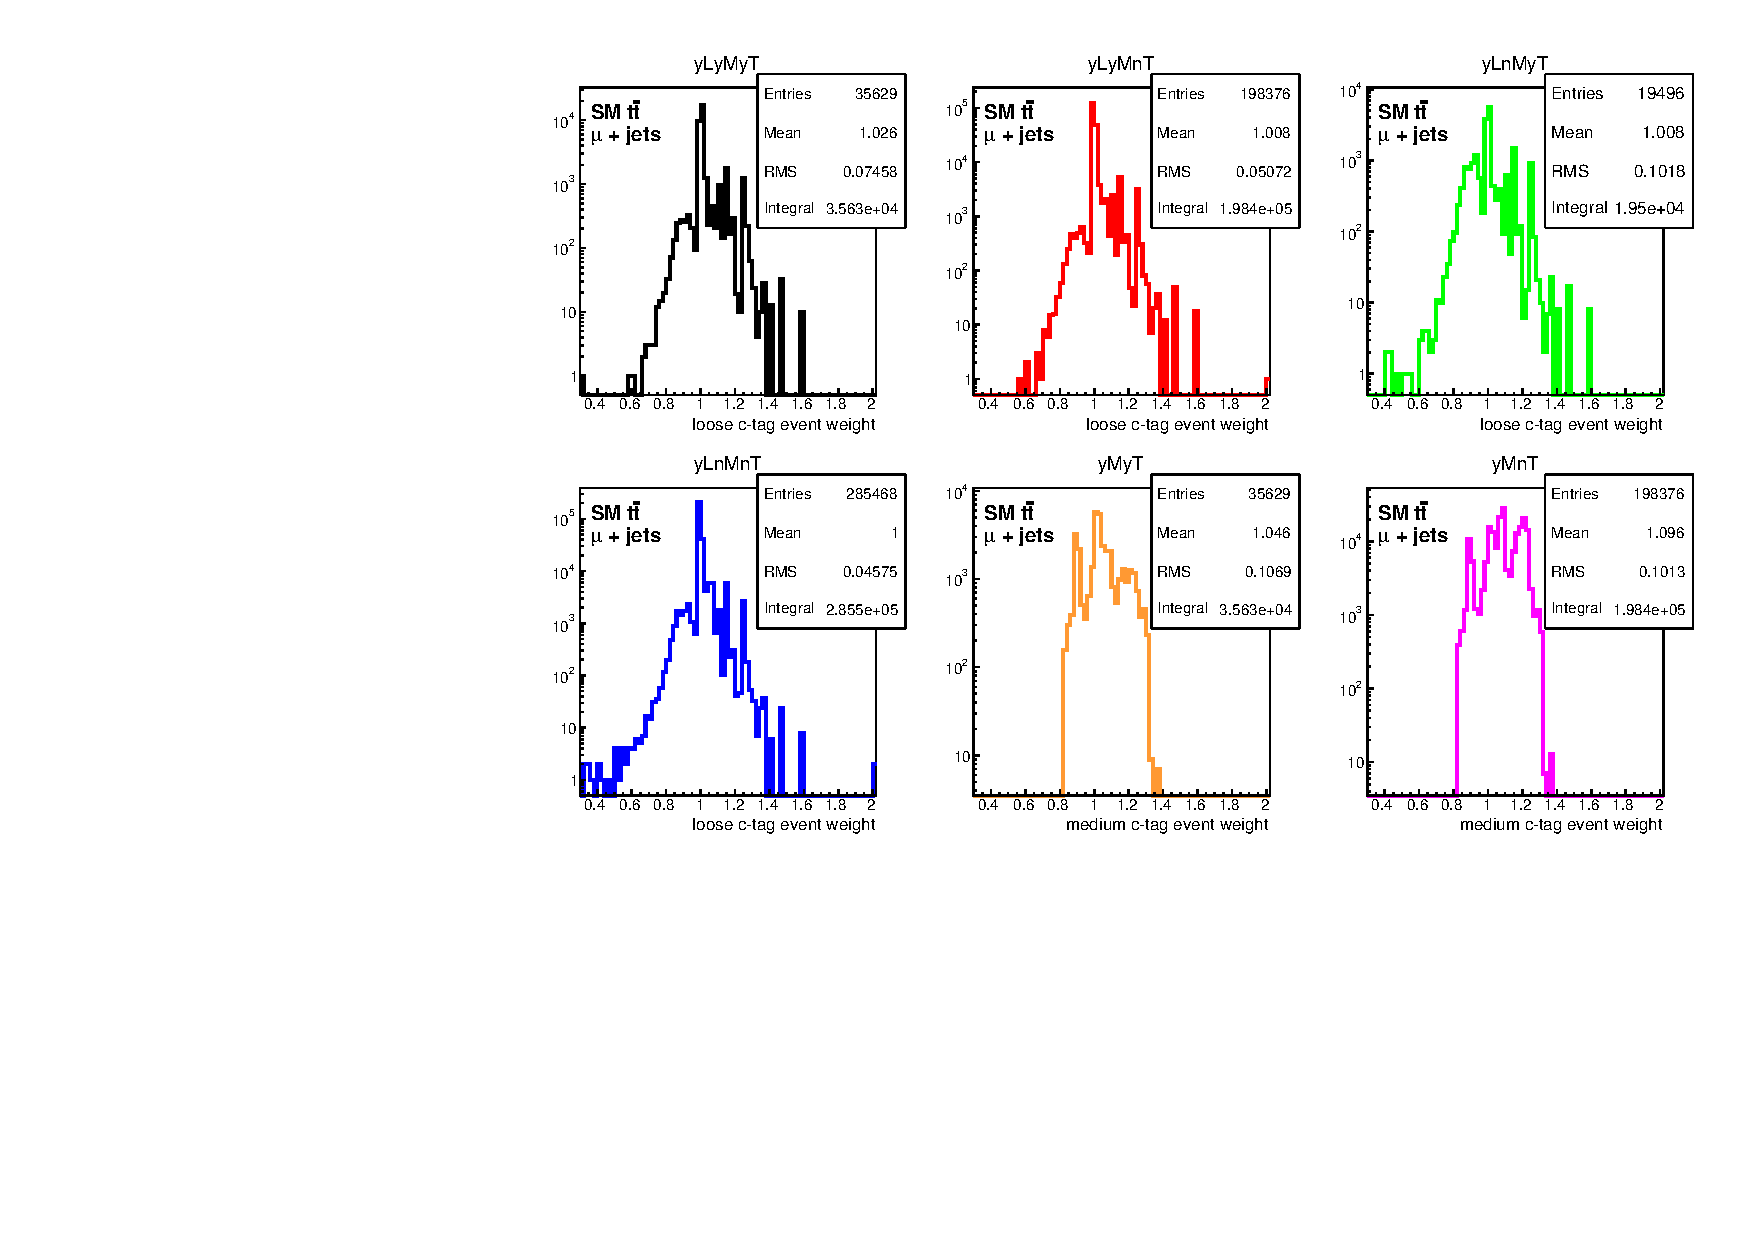
\includegraphics[width=0.90\linewidth]{Image/Muon/CTag/muExtraNP.pdf}}
    \vfil
    \subfigure[\label{subfig:extraNPele}]
    {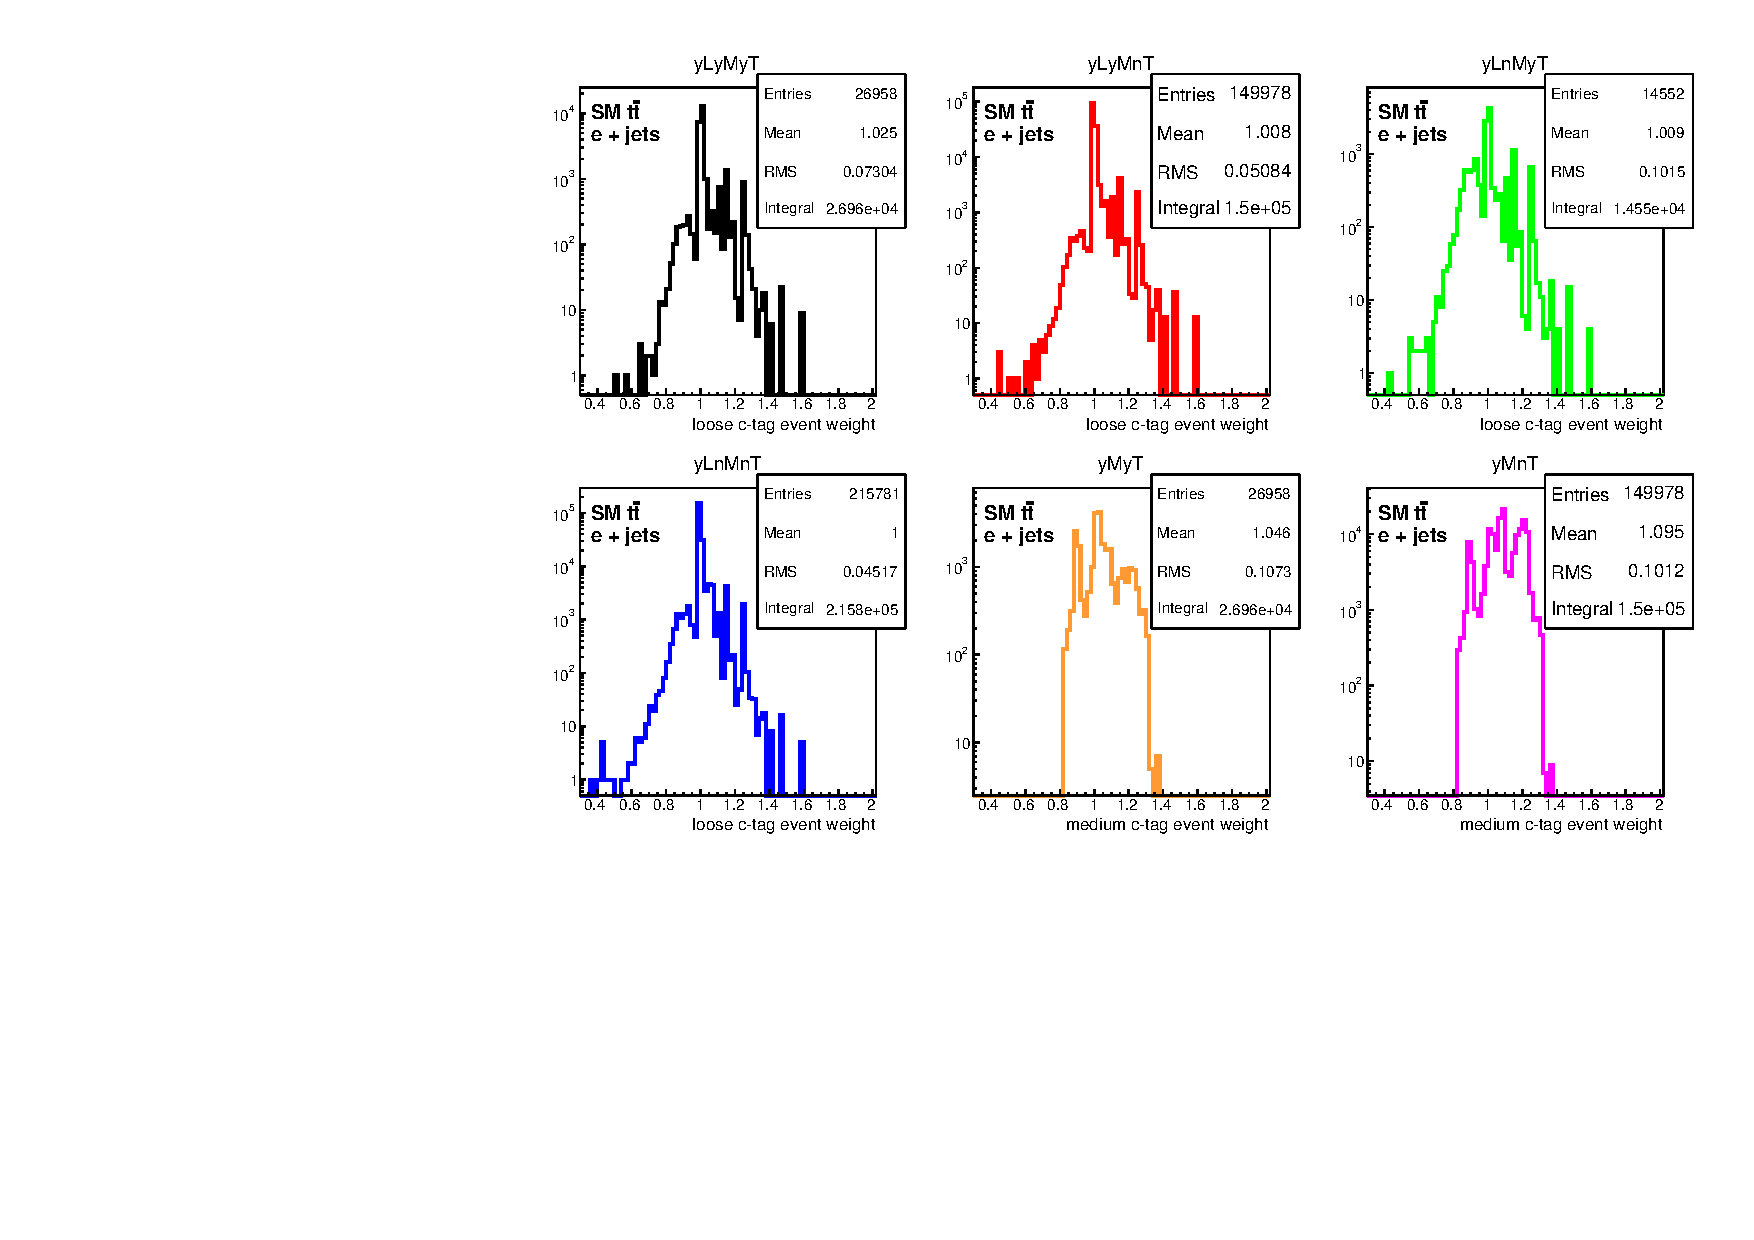
\includegraphics[width=0.90\linewidth]{Image/Electron/CTag/eleExtraNP.pdf}}
    \caption{The \PQc tag event weight for different cases from \ttjets 
        sample for both channels. For exclusive loose charm category, the value of 
        $CMS\_eff\_ExL$ = 1.026/0.9961 (1.025/0.9960) for \mujets
        (\ejets) channel. For exclusive medium charm category, the value of
        $CMS\_eff\_ExM$ = 1.096/1.046 (1.095/1.046) for \mujets (\ejets) channel.}
    \label{fig:extraNP}
\end{figure}

\item {\bf {QCD multijet data-driven uncertainty}}: The relative isolation of muon (electron) 
	are conservatively shifted to 0.17 (0.11) and the corresponding change in the 
	QCD multijet yield is determined. The percentage change in the yield is considered as 
	systematic uncertainty in the QCD multijet estimation.
 
\item {\bf {Bin-by-bin uncertainty}}: In some of the bins of $\mjj$ distributions, 
	the statistics are small hence statistical uncertainty is large. In each bin of 
	summed $\mjj$ from all backgrounds, one shape nuisance parameter (as described in 
	Section~\ref{a:secShapeVslnN}) is considered.
\end{itemize}

\section{Theoretical uncertainties}
\begin{itemize}[leftmargin=*]
\item {\bf {Normalization}}: The uncertainty in the cross section of each simulated sample is 
	considered. 

\item {\bf {\PQt quark \pt re-weighting}}: The \PQt quark \pt weights are determined from 
	following equation
    \begin{equation}
    w_{\rm{top}}=\sqrt{\rm{SF(t)}\times \rm{SF}(\bar{\rm{t}})}, \quad\rm {where}\quad \rm{SF}\equiv\exp(0.0615 - 0.0005\times\pt).
    \label{eq:top_wt}
    \end{equation}
    The values in the exponent are given in \cite{CMS-PAS-TOP-16-011, CMS-PAS-TOP-16-008}.
    The generator level $\pt$ of \PQt and $\bar{\PQt}$ quark is used to calculate the SF. 
    The \textit{particle data group} code \dq{6} is used to identify \PQt quark at parton level. 
	The $w_{\rm{top}}$ is taken 
	to be 1 for \dq{down} and $w_{\rm{top}}^2$ for \dq{up} systematic. The \PQt quark \pt re-weighting 
	is applied only on \ttjets and charged Higgs samples shown in Table~\ref{tab:mcSample}. The 
	effect of \PQt quark \pt re-weighting on the $\mjj$ is shown in 
	Figures~\ref{subfig:sys_topPt_wh_mu},~\ref{subfig:sys_topPt_wh_ele}, for charged Higgs 
	signal ($\mHp = 120$ \GeV) and in Figures~\ref{subfig:sys_topPt_ttbar_mu}, 
	\ref{subfig:sys_topPt_ttbar_ele} for \ttjets background for both channels. 
\item {\bf {\PQt quark mass}}: The \ttjets sample shown in Table~\ref{tab:mcSample} was 
    generated with \mt =172.5 \GeV. We used \ttjets sample with \mt =171.5 
    \GeV and \mt =173.5 \GeV, as shown in Table~\ref{tab:mcSampleSys}, to observe the 
    effect of \PQt quark mass on the $\mjj$. The $\mjj$ for different \mt are shown  
    in Figures~\ref{subfig:sys_mass_ttbar_mu},~\ref{subfig:sys_mass_ttbar_ele}
    for \ttjets background for both channels. 

\item {\bf {Parton shower matching}}: In the \POWHEG + \PYTHIA generated samples, the 
    next-to-leading order (NLO) matrix element parton shower matching is varied by $h_{\rm {damp}}$
    parameter. The \ttjets samples generated by varying $h_{\rm{damp}}$ \dq{up} and 
    \dq{down}, as shown in Table~\ref{tab:mcSampleSys} are used to see the effect of $h_{\rm{damp}}$ 
    on the $\mjj$ distribution as shown  
    in Figures~\ref{subfig:sys_matching_ttbar_mu},~\ref{subfig:sys_matching_ttbar_ele}
    for \ttjets background for both channels. 

\item {\bf {Renormalization and factorisation scale}}: To see the effect of renormalization and 
	factorisation scale, the \dq{up} and \dq{down} \ttjets samples as shown in 
	Table~\ref{tab:mcSampleSys} are used. The effect of these scales on the $\mjj$ are shown 
    	in Figures~\ref{subfig:sys_scale_ttbar_mu},~\ref{subfig:sys_scale_ttbar_ele} 
	for \ttjets background for both channels. 
\end{itemize}
The QCD multijet events are estimated from data. Hence none of the systematics 
(except the data-driven uncertainty) are considered on the QCD multijet background. 
The relative systematic and statistical uncertainties for all the process, from all event 
categories, and for both channels are shown in Tables~\ref{tab:sysInc}, \ref{tab:sysCTagInc}, 
and \ref{tab:sysCTagEx}.

\begin{table}
\caption{Systematic and statistical uncertainties in \%, from inclusive category after kinematic fit
selection for \mujets (\ejets) channel. The \dq{---} indicates that the corresponding uncertainties are not considered for the given process.}
\label{tab:sysInc}
\centering
\begin{adjustbox}{max width=\textwidth}
\begin{tabular}{  c c c c c c c c c c c c c cc}
\hline 
\hline 
Process &{\rotatebox{90}{Luminosity}} & {\rotatebox{90}{Pileup} } & {\rotatebox{90}{Lepton }} & {\rotatebox{90}{JES + JER + \MET}} & { \rotatebox{90}{\PQb \& \PQc tagging-1} }  & { \rotatebox{90}{\PQb \& \PQc tagging-2} } & { \rotatebox{90}{\PQb \& \PQc tagging-3}}& { \rotatebox{90}{Normalization}  }& {\rotatebox{90}{Statistical}  } & {\rotatebox{90}{\PQt quark \pt } }  \\ 
\hline 
\hline 
$\mHp=80$ GeV & 2.5 (2.5) &  0.86 (0.83) &  3.0 (3.0) & 6.1 (6.2) &  0.12 (0.089) &  0.33 (0.3) &  3.3 (3.3) &  6.1 (6.1) & 0.7 (0.8) & 1.1 (1.3) \\ 
$\mHp=90$ GeV & 2.5 (2.5) &  1 (0.93) &  3.0 (3.0) & 6.7 (6.4) &  0.012 (0.075) &  0.35 (0.43) &  3.4 (3.2) &  6.1 (6.1) & 0.69 (0.79) & 0.83 (1.7) \\ 
$\mHp=100$ GeV & 2.5 (2.5) &  0.77 (0.9) &  3.0 (3.0) & 6.3 (5.7) &  0.12 (0.14) &  0.3 (0.21) &  3.5 (3.2) &  6.1 (6.1) & 0.68 (0.78) & 0.6 (1.3) \\ 
$\mHp=120$ GeV & 2.5 (2.5) &  0.74 (1.3) &  3.0 (3.0) & 6.1 (5.9) &  0.31 (0.058) &  0.57 (0.5) &  3.4 (3.4) &  6.1 (6.1) & 0.69 (0.79) & 0.64 (1.2) \\ 
$\mHp=140$ GeV & 2.5 (2.5) &  0.83 (1.1) &  3.0 (3.0) & 6.7 (6.5) &  0.45 (0.031) &  0.28 (0.56) &  4 (3.6) &  6.1 (6.1) & 0.78 (0.88) & 1.2 (1.9) \\ 
$\mHp=150$ GeV & 2.5 (2.5) &  0.49 (0.87) &  3.0 (3.0) & 7.4 (7.6) &  0.24 (0.017) &  0.69 (0.75) &  4 (3.9) &  6.1 (6.1) & 0.92 (1) & 2 (3) \\ 
$\mHp=155$ GeV & 2.5 (2.5) &  0.97 (0.57) &  3.0 (3.0) & 8.8 (9.4) &  0.44 (0.24) &  1.3 (0.72) &  4.2 (4.1) &  6.1 (6.1) & 1.1 (1.2) & 2.4 (3.3) \\ 
$\mHp=160$ GeV & 2.5 (2.5) &  0.27 (0.81) &  3.0 (3.0) & 9 (9.4) &  0.59 (0.23) &  1.3 (1.1) &  4.1 (3.9) &  6.1 (6.1) & 1.2 (1.3) & 3.3 (3.4) \\ 
\hline 
SM \ttjets & 2.5 (2.5) &  0.74 (0.88) &  3.0 (3.0) & 6.6 (6.5) &  0.18 (0.019) &  0.43 (0.35) &  3.2 (3.1) &  6.1 (6.1) & 0.14 (0.16) & 0.68 (1.4) \\ 
Single \PQt & 2.5 (2.5) &  0.44 (0.59) &  3.0 (3.0) & 8.8 (9.4) &  0.39 (0.14) &  0.8 (0.84) &  3.5 (3.5) &  5 (5) & 0.76 (0.87) & --- \\ 
\wjets & 2.5 (2.5) &  1 (0.81) &  3.0 (3.0) & 19 (13) &  1.2 (0.079) &  4.4 (3.5) &  6.7 (4.6) &  5 (5) & 4.4 (3.5) & --- \\ 
\dyjets & 2.5 (2.5) &  1.4 (3) &  3.0 (3.0) & 18 (16) &  1.7 (0.12) &  4.3 (3.7) &  5.3 (3.8) &  4.5 (4.5) & 3.9 (3.4) & --- \\ 
VV & 2.5 (2.5) &  5 (6.5) &  3.0 (3.0) & 17 (17) &  6.4 (3.3) &  8.2 (3.7) &  6 (5.8) &  4 (4) & 14 (19) & --- \\ 
QCD multijet & --- &  --- &  --- & --- &  --- &  --- &  --- &  13 (18) & 5.2 (4.7) & --- \\ 
\hline 

\end{tabular}
\end{adjustbox}
\end{table}

\begin{table}
\caption{Systematic and statistical uncertainties in \%, from inclusive loose charm tagging category
after kinematic fit selection for \mujets (\ejets) channel. The \dq{---} indicates that the corresponding uncertainties are not considered for the given process.}
\label{tab:sysCTagInc}
\centering
\begin{adjustbox}{max width=\textwidth}
\begin{tabular}{  c c c c c c c c c c c c c cc}
\hline 
\hline 
Process &{\rotatebox{90}{Luminosity}} & {\rotatebox{90}{Pileup} } & {\rotatebox{90}{Lepton }} & {\rotatebox{90}{JES + JER + \MET}} & { \rotatebox{90}{\PQb \& \PQc tagging-1} }  & { \rotatebox{90}{\PQb \& \PQc tagging-2} } & { \rotatebox{90}{\PQb \& \PQc tagging-3}}& { \rotatebox{90}{Normalization}  }& {\rotatebox{90}{Statistical}  } & {\rotatebox{90}{\PQt quark \pt } }  \\ 
\hline 
\hline 
$\mHp=80$ GeV & 2.5 (2.5) &  0.88 (0.82) &  3.0 (3.0) & 6.1 (6) &  2 (2) &  4 (4) &  4.7 (4.7) &  6.1 (6.1) & 0.71 (0.81) & 1.1 (1.3) \\ 
$\mHp=90$ GeV & 2.5 (2.5) &  1.1 (0.95) &  3.0 (3.0) & 6.7 (6.5) &  1.6 (1.4) &  4.1 (4.2) &  4.8 (4.5) &  6.1 (6.1) & 0.7 (0.79) & 0.84 (1.7) \\ 
$\mHp=100$ GeV & 2.5 (2.5) &  0.77 (0.89) &  3.0 (3.0) & 6.3 (5.7) &  1.8 (2.5) &  3.9 (3.9) &  4.9 (4.7) &  6.1 (6.1) & 0.68 (0.78) & 0.59 (1.2) \\ 
$\mHp=120$ GeV & 2.5 (2.5) &  0.72 (1.3) &  3.0 (3.0) & 5.9 (5.9) &  1.6 (1.6) &  4.3 (4.2) &  5.2 (5.1) &  6.1 (6.1) & 0.7 (0.8) & 0.65 (1.1) \\ 
$\mHp=140$ GeV & 2.5 (2.5) &  0.88 (1.1) &  3.0 (3.0) & 6.7 (6.5) &  2.1 (1.5) &  4 (4.2) &  6.1 (5.5) &  6.1 (6.1) & 0.79 (0.89) & 1.1 (1.9) \\ 
$\mHp=150$ GeV & 2.5 (2.5) &  0.5 (0.87) &  3.0 (3.0) & 7.4 (7.6) &  2 (1.7) &  4.5 (4.5) &  6 (5.9) &  6.1 (6.1) & 0.93 (1) & 2 (3) \\ 
$\mHp=155$ GeV & 2.5 (2.5) &  1.1 (0.58) &  3.0 (3.0) & 8.8 (9.4) &  2.6 (1.8) &  5.3 (4.7) &  6.8 (6.4) &  6.1 (6.1) & 1.1 (1.2) & 2.4 (3.3) \\ 
$\mHp=160$ GeV & 2.5 (2.5) &  0.37 (0.84) &  3.0 (3.0) & 9 (9.3) &  1.3 (1.5) &  5.2 (5) &  6.3 (6.1) &  6.1 (6.1) & 1.2 (1.3) & 3.3 (3.4) \\ 
\hline 
SM \ttjets & 2.5 (2.5) &  0.74 (0.89) &  3.0 (3.0) & 6.5 (6.5) &  1.1 (0.9) &  4.6 (4.5) &  4.2 (4.1) &  6.1 (6.1) & 0.14 (0.16) & 0.68 (1.4) \\ 
Single \PQt & 2.5 (2.5) &  0.46 (0.62) &  3.0 (3.0) & 8.7 (9.3) &  1 (0.78) &  5.1 (5.3) &  4.6 (4.7) &  5 (5) & 0.76 (0.88) & --- \\ 
\wjets & 2.5 (2.5) &  0.94 (0.68) &  3.0 (3.0) & 19 (13) &  1.7 (0.37) &  9.3 (8.4) &  7.6 (5.7) &  5 (5) & 4.4 (3.5) & --- \\ 
\dyjets & 2.5 (2.5) &  1.2 (2.8) &  3.0 (3.0) & 19 (16) &  1.4 (0.31) &  9 (8.2) &  6.9 (5.6) &  4.5 (4.5) & 4 (3.6) & --- \\ 
VV & 2.5 (2.5) &  4.9 (6.4) &  3.0 (3.0) & 17 (16) &  5.9 (4.2) &  11 (7.8) &  7.1 (6.2) &  4 (4) & 14 (19) & --- \\ 
QCD multijet & --- &  --- &  --- & --- &  --- &  --- &  --- &  14 (21) & 5.4 (5) & --- \\ 
\hline 
\end{tabular}
\end{adjustbox}
\end{table}

\begin{table}
\caption{Systematic and statistical uncertainties in \%, from exclusive charm tagging categories after 
kinematic fit selection for \mujets (\ejets) channel. The \dq{---} indicates that the corresponding 
uncertainties are not considered for the given process.}
\label{tab:sysCTagEx}
\centering
\begin{adjustbox}{max width=\textwidth}
\begin{tabular}{c  c c c c c c c c c c c c c cc}
\hline 
\hline 
Category & Process &{\rotatebox{90}{Luminosity}} & {\rotatebox{90}{Pileup} } & {\rotatebox{90}{Lepton }} & {\rotatebox{90}{JES + JER + \MET}} & { \rotatebox{90}{\PQb \& \PQc tagging-1} }  & { \rotatebox{90}{\PQb \& \PQc tagging-2} } & { \rotatebox{90}{\PQb \& \PQc tagging-3}}& { \rotatebox{90}{Normalization}  }& {\rotatebox{90}{Statistical}  } & {\rotatebox{90}{\PQt quark \pt } }  \\ 
\hline 
\hline 
Loose  & $\mHp=80$ GeV & 2.5 (2.5) &  0.96 (0.94) &  3.0 (3.0) & 6.8 (6.7) &  1.6 (1.8) &  4.5 (4.1) &  4.4 (4.3) &  6.1 (6.1) & 1 (1.2) & 0.86 (1.2) \\ 
       & $\mHp=90$ GeV & 2.5 (2.5) &  1.2 (0.88) &  3.0 (3.0) & 7.5 (7.1) &  1.3 (1.2) &  4.5 (4.5) &  4.4 (4.3) &  6.1 (6.1) & 1 (1.2) & 0.78 (1.4) \\ 
       & $\mHp=100$ GeV & 2.5 (2.5) &  0.81 (1.2) &  3.0 (3.0) & 7.4 (6.8) &  1.5 (2.1) &  4.2 (4.2) &  4.4 (4.3) &  6.1 (6.1) & 1 (1.2) & 0.49 (1) \\ 
       & $\mHp=120$ GeV & 2.5 (2.5) &  0.86 (1.4) &  3.0 (3.0) & 6.9 (7.3) &  1.4 (1.1) &  4.7 (4.3) &  4.7 (4.6) &  6.1 (6.1) & 1 (1.2) & 0.49 (1.3) \\ 
       & $\mHp=140$ GeV & 2.5 (2.5) &  0.9 (1.4) &  3.0 (3.0) & 7.8 (7.1) &  1.8 (1.1) &  4.2 (4.4) &  5.9 (5.2) &  6.1 (6.1) & 1.2 (1.3) & 1.3 (1.7) \\ 
       & $\mHp=150$ GeV & 2.5 (2.5) &  0.65 (0.96) &  3.0 (3.0) & 7.7 (7.8) &  2.1 (1.6) &  4.9 (4.6) &  6.1 (5.7) &  6.1 (6.1) & 1.3 (1.5) & 1.9 (3) \\ 
       & $\mHp=155$ GeV & 2.5 (2.5) &  1.3 (0.59) &  3.0 (3.0) & 8.8 (10) &  1.5 (1.6) &  4.7 (4.9) &  5.7 (6.2) &  6.1 (6.1) & 1.5 (1.8) & 3 (3.1) \\ 
       & $\mHp=160$ GeV & 2.5 (2.5) &  0.91 (1.2) &  3.0 (3.0) & 9.3 (8.9) &  0.83 (1) &  4.8 (5.1) &  5.3 (5.6) &  6.1 (6.1) & 1.7 (1.9) & 2.7 (2.8) \\ 
       & SM \ttjets & 2.5 (2.5) &  0.97 (1.2) &  3.0 (3.0) & 6.9 (6.9) &  0.74 (0.58) &  4.5 (4.5) &  3.8 (3.7) &  6.1 (6.1) & 0.19 (0.22) & 0.73 (1.3) \\ 
       & Single \PQt  & 2.5 (2.5) &  1.1 (0.82) &  3.0 (3.0) & 9.1 (10) &  0.73 (0.63) &  5 (5.2) &  4.5 (4.2) &  5 (5) & 1 (1.2) & --- \\ 
       & \wjets & 2.5 (2.5) &  1.4 (1.1) &  3.0 (3.0) & 18 (13) &  1.2 (0.29) &  10 (8.3) &  9.8 (5.1) &  5 (5) & 6.8 (4.6) & --- \\ 
       & \dyjets & 2.5 (2.5) &  0.4 (2.3) &  3.0 (3.0) & 20 (18) &  1.5 (0.44) &  8.7 (8.2) &  6.9 (4.4) &  4.5 (4.5) & 5.9 (4.4) & --- \\ 
       & VV & 2.5 (2.5) &  4.5 (11) &  3.0 (3.0) & 8.7 (16) &  2.1 (4) &  6.5 (8.5) &  7.3 (7.2) &  4 (4) & 21 (22) & --- \\ 
       & QCD multijet & --- &  --- &  --- & --- &  --- &  --- &  --- &  13 (23) & 7.9 (7.7) & --- \\ 
\hline   
Medium & $\mHp=80$ GeV & 2.5 (2.5) &  1.1 (0.55) &  3.0 (3.0) & 5.6 (6.1) &  3 (2.9) &  5 (4.9) &  3.6 (3.7) &  6.1 (6.1) & 1.2 (1.3) & 1.3 (1.5) \\ 
       & $\mHp=90$ GeV & 2.5 (2.5) &  0.88 (0.69) &  3.0 (3.0) & 6.5 (6.3) &  3 (2.8) &  5 (5.4) &  3.8 (3.8) &  6.1 (6.1) & 1.1 (1.3) & 0.77 (1.9) \\ 
       & $\mHp=100$ GeV & 2.5 (2.5) &  0.65 (0.36) &  3.0 (3.0) & 6.7 (4.8) &  2.8 (2.7) &  5 (4.9) &  3.9 (3.8) &  6.1 (6.1) & 1.1 (1.3) & 0.65 (1.5) \\ 
       & $\mHp=120$ GeV & 2.5 (2.5) &  0.63 (0.83) &  3.0 (3.0) & 5.9 (5.1) &  2.8 (2.8) &  5.2 (5) &  4.2 (3.8) &  6.1 (6.1) & 1.1 (1.3) & 0.63 (1.2) \\ 
       & $\mHp=140$ GeV & 2.5 (2.5) &  0.6 (0.89) &  3.0 (3.0) & 6.2 (6.8) &  3.3 (2.9) &  5.2 (5.6) &  4.9 (4.4) &  6.1 (6.1) & 1.3 (1.4) & 0.78 (2.3) \\ 
       & $\mHp=150$ GeV & 2.5 (2.5) &  0.98 (0.73) &  3.0 (3.0) & 8 (7.7) &  2.3 (2.7) &  5.5 (5.7) &  4.7 (4.5) &  6.1 (6.1) & 1.5 (1.7) & 2.1 (3.2) \\ 
       & $\mHp=155$ GeV & 2.5 (2.5) &  0.45 (0.48) &  3.0 (3.0) & 8.7 (10) &  3.1 (2.6) &  7 (5.7) &  5.5 (4.9) &  6.1 (6.1) & 1.8 (1.9) & 1.8 (3.1) \\ 
       & $\mHp=160$ GeV & 2.5 (2.5) &  0.2 (0.37) &  3.0 (3.0) & 9.4 (11) &  2.1 (2.6) &  6.9 (5.9) &  5.2 (4.9) &  6.1 (6.1) & 1.9 (2.2) & 3.3 (4) \\ 
       & SM \ttjets & 2.5 (2.5) &  0.25 (0.45) &  3.0 (3.0) & 6.2 (6.2) &  1.8 (1.6) &  6.3 (6.2) &  3.4 (3.5) &  6.1 (6.1) & 0.23 (0.27) & 0.62 (1.4) \\ 
       & Single \PQt  & 2.5 (2.5) &  0.73 (0.29) &  3.0 (3.0) & 8.5 (8.6) &  1.6 (1.3) &  7 (7.2) &  3.4 (3.9) &  5 (5) & 1.3 (1.5) & --- \\ 
       & \wjets & 2.5 (2.5) &  1.5 (2.5) &  3.0 (3.0) & 21 (12) &  2.1 (1.6) &  11 (11) &  5.1 (5.4) &  5 (5) & 5 (5.8) & --- \\ 
       & \dyjets & 2.5 (2.5) &  1.5 (3.5) &  3.0 (3.0) & 21 (17) &  2 (0.51) &  11 (11) &  4.2 (5.2) &  4.5 (4.5) & 6.3 (6) & --- \\ 
       & VV & 2.5 (2.5) &  13 (7.2) &  3.0 (3.0) & 28 (54) &  5.1 (6.4) &  20 (8.3) &  8.9 (3.2) &  4 (4) & 21 (35) & --- \\ 
       & QCD multijet & --- &  --- &  --- & --- &  --- &  --- &  --- &  15 (16) & 12 (10) & --- \\ 
\hline   
Tight  & $\mHp=80$ GeV & 2.5 (2.5) &  0.65 (1.4) &  3.0 (3.0) & 5.6 (4.4) &  5.7 (6.2) &  4.5 (5.5) &  6.3 (5.8) &  6.1 (6.1) & 1.7 (2) & 1.1 (0.78) \\ 
       & $\mHp=90$ GeV & 2.5 (2.5) &  1.2 (1.6) &  3.0 (3.0) & 5.8 (5.4) &  5.5 (6.4) &  5.8 (5) &  5.1 (5.1) &  6.1 (6.1) & 1.7 (2) & 0.92 (1.9) \\ 
       & $\mHp=100$ GeV & 2.5 (2.5) &  1.3 (1.4) &  3.0 (3.0) & 5.2 (5.6) &  6.1 (5.9) &  5.5 (5) &  5.6 (5.3) &  6.1 (6.1) & 1.7 (1.9) & 0.85 (1.1) \\ 
       & $\mHp=120$ GeV & 2.5 (2.5) &  1 (1.7) &  3.0 (3.0) & 4.8 (4.5) &  5.6 (5.9) &  5.2 (5.4) &  5.4 (5.9) &  6.1 (6.1) & 1.7 (1.9) & 0.95 (0.59) \\ 
       & $\mHp=140$ GeV & 2.5 (2.5) &  1.1 (1.6) &  3.0 (3.0) & 5.5 (4.8) &  6.3 (6.4) &  4.7 (5.3) &  5.3 (5.7) &  6.1 (6.1) & 2 (2.2) & 1.6 (1.1) \\ 
       & $\mHp=150$ GeV & 2.5 (2.5) &  0.84 (1.8) &  3.0 (3.0) & 6.3 (7.7) &  7.1 (6) &  5.2 (5.9) &  5.9 (6.3) &  6.1 (6.1) & 2.4 (2.6) & 1.9 (2.2) \\ 
       & $\mHp=155$ GeV & 2.5 (2.5) &  2.1 (1.1) &  3.0 (3.0) & 9.3 (6) &  7.3 (6.1) &  7.3 (5.5) &  7.5 (6.4) &  6.1 (6.1) & 2.8 (3.1) & 1.9 (4.5) \\ 
       & $\mHp=160$ GeV & 2.5 (2.5) &  0.63 (1.5) &  3.0 (3.0) & 8.9 (6.9) &  7.1 (5.8) &  5.7 (6.3) &  7.2 (5.6) &  6.1 (6.1) & 3.3 (3.8) & 4.9 (3.6) \\ 
       & SM \ttjets & 2.5 (2.5) &  1.3 (0.93) &  3.0 (3.0) & 5.9 (6) &  4.9 (4.9) &  6.8 (6.3) &  5.5 (5.1) &  6.1 (6.1) & 0.44 (0.5) & 0.47 (1.3) \\ 
       & Single \PQt  & 2.5 (2.5) &  0.72 (0.38) &  3.0 (3.0) & 7.8 (8.9) &  4.7 (4.2) &  7.6 (7) &  6.2 (5.8) &  5 (5) & 2.6 (3) & --- \\ 
       & \wjets & 2.5 (2.5) &  2.4 (3) &  3.0 (3.0) & 23 (27) &  9.7 (5.4) &  9.2 (9.5) &  13 (7.9) &  5 (5) & 13 (14) & --- \\ 
       & \dyjets & 2.5 (2.5) &  8.8 (4.6) &  3.0 (3.0) & 8.6 (13) &  4.5 (3.6) &  16 (9.5) &  10 (8.1) &  4.5 (4.5) & 9.5 (15) & --- \\ 
       & VV & 2.5 (2.5) &  0.66 (8.9) &  3.0 (3.0) & 27 (0) &  32 (7.4) &  9.1 (6.9) &  10 (2.3) &  4 (4) & 40 (1e+02) & --- \\ 
       & QCD multijet & --- &  --- &  --- & --- &  --- &  --- &  --- &   11 (13) & 28 (18) & --- \\ 
\hline 
\end{tabular}
\end{adjustbox}
\end{table}
